\PassOptionsToPackage{unicode=true}{hyperref} % options for packages loaded elsewhere
\PassOptionsToPackage{hyphens}{url}
%
\documentclass[]{book}
\usepackage{lmodern}
\usepackage{amssymb,amsmath}
\usepackage{ifxetex,ifluatex}
\usepackage{fixltx2e} % provides \textsubscript
\ifnum 0\ifxetex 1\fi\ifluatex 1\fi=0 % if pdftex
  \usepackage[T1]{fontenc}
  \usepackage[utf8]{inputenc}
  \usepackage{textcomp} % provides euro and other symbols
\else % if luatex or xelatex
  \usepackage{unicode-math}
  \defaultfontfeatures{Ligatures=TeX,Scale=MatchLowercase}
\fi
% use upquote if available, for straight quotes in verbatim environments
\IfFileExists{upquote.sty}{\usepackage{upquote}}{}
% use microtype if available
\IfFileExists{microtype.sty}{%
\usepackage[]{microtype}
\UseMicrotypeSet[protrusion]{basicmath} % disable protrusion for tt fonts
}{}
\IfFileExists{parskip.sty}{%
\usepackage{parskip}
}{% else
\setlength{\parindent}{0pt}
\setlength{\parskip}{6pt plus 2pt minus 1pt}
}
\usepackage{hyperref}
\hypersetup{
            pdftitle={I am Bilingual - Python and R},
            pdfauthor={Priyanga Dilini Talagala   Thiyanga S. Talagala},
            pdfborder={0 0 0},
            breaklinks=true}
\urlstyle{same}  % don't use monospace font for urls
\usepackage{color}
\usepackage{fancyvrb}
\newcommand{\VerbBar}{|}
\newcommand{\VERB}{\Verb[commandchars=\\\{\}]}
\DefineVerbatimEnvironment{Highlighting}{Verbatim}{commandchars=\\\{\}}
% Add ',fontsize=\small' for more characters per line
\usepackage{framed}
\definecolor{shadecolor}{RGB}{248,248,248}
\newenvironment{Shaded}{\begin{snugshade}}{\end{snugshade}}
\newcommand{\AlertTok}[1]{\textcolor[rgb]{0.94,0.16,0.16}{#1}}
\newcommand{\AnnotationTok}[1]{\textcolor[rgb]{0.56,0.35,0.01}{\textbf{\textit{#1}}}}
\newcommand{\AttributeTok}[1]{\textcolor[rgb]{0.77,0.63,0.00}{#1}}
\newcommand{\BaseNTok}[1]{\textcolor[rgb]{0.00,0.00,0.81}{#1}}
\newcommand{\BuiltInTok}[1]{#1}
\newcommand{\CharTok}[1]{\textcolor[rgb]{0.31,0.60,0.02}{#1}}
\newcommand{\CommentTok}[1]{\textcolor[rgb]{0.56,0.35,0.01}{\textit{#1}}}
\newcommand{\CommentVarTok}[1]{\textcolor[rgb]{0.56,0.35,0.01}{\textbf{\textit{#1}}}}
\newcommand{\ConstantTok}[1]{\textcolor[rgb]{0.00,0.00,0.00}{#1}}
\newcommand{\ControlFlowTok}[1]{\textcolor[rgb]{0.13,0.29,0.53}{\textbf{#1}}}
\newcommand{\DataTypeTok}[1]{\textcolor[rgb]{0.13,0.29,0.53}{#1}}
\newcommand{\DecValTok}[1]{\textcolor[rgb]{0.00,0.00,0.81}{#1}}
\newcommand{\DocumentationTok}[1]{\textcolor[rgb]{0.56,0.35,0.01}{\textbf{\textit{#1}}}}
\newcommand{\ErrorTok}[1]{\textcolor[rgb]{0.64,0.00,0.00}{\textbf{#1}}}
\newcommand{\ExtensionTok}[1]{#1}
\newcommand{\FloatTok}[1]{\textcolor[rgb]{0.00,0.00,0.81}{#1}}
\newcommand{\FunctionTok}[1]{\textcolor[rgb]{0.00,0.00,0.00}{#1}}
\newcommand{\ImportTok}[1]{#1}
\newcommand{\InformationTok}[1]{\textcolor[rgb]{0.56,0.35,0.01}{\textbf{\textit{#1}}}}
\newcommand{\KeywordTok}[1]{\textcolor[rgb]{0.13,0.29,0.53}{\textbf{#1}}}
\newcommand{\NormalTok}[1]{#1}
\newcommand{\OperatorTok}[1]{\textcolor[rgb]{0.81,0.36,0.00}{\textbf{#1}}}
\newcommand{\OtherTok}[1]{\textcolor[rgb]{0.56,0.35,0.01}{#1}}
\newcommand{\PreprocessorTok}[1]{\textcolor[rgb]{0.56,0.35,0.01}{\textit{#1}}}
\newcommand{\RegionMarkerTok}[1]{#1}
\newcommand{\SpecialCharTok}[1]{\textcolor[rgb]{0.00,0.00,0.00}{#1}}
\newcommand{\SpecialStringTok}[1]{\textcolor[rgb]{0.31,0.60,0.02}{#1}}
\newcommand{\StringTok}[1]{\textcolor[rgb]{0.31,0.60,0.02}{#1}}
\newcommand{\VariableTok}[1]{\textcolor[rgb]{0.00,0.00,0.00}{#1}}
\newcommand{\VerbatimStringTok}[1]{\textcolor[rgb]{0.31,0.60,0.02}{#1}}
\newcommand{\WarningTok}[1]{\textcolor[rgb]{0.56,0.35,0.01}{\textbf{\textit{#1}}}}
\usepackage{longtable,booktabs}
% Fix footnotes in tables (requires footnote package)
\IfFileExists{footnote.sty}{\usepackage{footnote}\makesavenoteenv{longtable}}{}
\usepackage{graphicx,grffile}
\makeatletter
\def\maxwidth{\ifdim\Gin@nat@width>\linewidth\linewidth\else\Gin@nat@width\fi}
\def\maxheight{\ifdim\Gin@nat@height>\textheight\textheight\else\Gin@nat@height\fi}
\makeatother
% Scale images if necessary, so that they will not overflow the page
% margins by default, and it is still possible to overwrite the defaults
% using explicit options in \includegraphics[width, height, ...]{}
\setkeys{Gin}{width=\maxwidth,height=\maxheight,keepaspectratio}
\setlength{\emergencystretch}{3em}  % prevent overfull lines
\providecommand{\tightlist}{%
  \setlength{\itemsep}{0pt}\setlength{\parskip}{0pt}}
\setcounter{secnumdepth}{5}
% Redefines (sub)paragraphs to behave more like sections
\ifx\paragraph\undefined\else
\let\oldparagraph\paragraph
\renewcommand{\paragraph}[1]{\oldparagraph{#1}\mbox{}}
\fi
\ifx\subparagraph\undefined\else
\let\oldsubparagraph\subparagraph
\renewcommand{\subparagraph}[1]{\oldsubparagraph{#1}\mbox{}}
\fi

% set default figure placement to htbp
\makeatletter
\def\fps@figure{htbp}
\makeatother

\usepackage{booktabs}
\usepackage{amsthm}
\makeatletter
\def\thm@space@setup{%
  \thm@preskip=8pt plus 2pt minus 4pt
  \thm@postskip=\thm@preskip
}
\makeatother
\usepackage[]{natbib}
\bibliographystyle{apalike}

\title{I am Bilingual - Python and R}
\author{Priyanga Dilini Talagala Thiyanga S. Talagala}
\date{2021-04-26}

\begin{document}
\maketitle

{
\setcounter{tocdepth}{1}
\tableofcontents
}
\hypertarget{preface}{%
\chapter*{Preface}\label{preface}}
\addcontentsline{toc}{chapter}{Preface}

WIP!!

\textbf{This book is still in progress in various draft forms.}

\hypertarget{intro}{%
\chapter{Introduction to R and Python}\label{intro}}

WIP

\hypertarget{about-r-and-python}{%
\section{About R and Python}\label{about-r-and-python}}

\hypertarget{r}{%
\subsection{R}\label{r}}

R is an object oriented, open source programming \textbf{language} and \textbf{environment} for statistical computing and graphics. R is not a statistics system but an environment within which statistical techniques are implemented. Further, R gains more capabilities via packages, its fundamental shareable units that bundle together R functions, code, data, documentation, and tests etc. \citep{Rcoreteam2020}.

\hypertarget{python}{%
\subsection{Python}\label{python}}

Python is an object-oriented, interpreted, and interactive programming language. The motto of Python language is ``Batteries included'' as the functionality of the language can be performed via its comprehensive standard in built Libraries \citep{wikipython}.

\hypertarget{history-of-r-and-python}{%
\section{History of R and Python}\label{history-of-r-and-python}}

\hypertarget{r-1}{%
\subsection{R}\label{r-1}}

R is an implementation of the S programming language which was created by John Chambers in 1976. In 1991, an alternative implementation of the basic S language was developed by Ross Ihaka and Robert Gentleman, University of Auckland, New Zealand. It was published in 1993 \citep{wikiR}.

\hypertarget{python-1}{%
\subsection{Python}\label{python-1}}

In 1989, Guido van Rossum at Centrum Wiskunde \& Informatica (CWI) in the Netherlands started the implementation of Python as a successor to ABC programming language. Python 2.0 was released in 2000. Python 3.0, a major revision of the language that is not completely backward-compatible was released in 2008 \citep{wikipython} . Today many developers create libraries strictly for the use with Python 3.

\hypertarget{story-behind-their-names}{%
\section{Story behind their names}\label{story-behind-their-names}}

\hypertarget{r-2}{%
\subsection{R}\label{r-2}}

R was introduced by \textbf{R}oss Ihaka and \textbf{R}obert Gentleman and it was named after the first names of the two authors. The name of the ``S'' language also had some influence on the selection of its name and it was selected partly as a play on the name of S \citep{wikiR}.

\hypertarget{python-2}{%
\subsection{Python}\label{python-2}}

Python was named after a famous \href{https://en.wikipedia.org/wiki/Monty_Python\%27s_Flying_Circus}{TV show `Monty Python's Flying Circus'}. Guido van Rossum, the creater of Python was a big fan of the TV show. He wanted to name his invention with a short, unique and slightly mysterious name and chose Python as a working title for his ongoing project.

\hypertarget{logo}{%
\section{Logo}\label{logo}}

\begin{figure}

{\centering 
\includegraphics[width=0.3\linewidth]{fig/C1_Rlogo} 

}

\caption{Retrieved from: https://www.r-project.org/logo/}\label{fig:unnamed-chunk-1}
\end{figure}

\begin{figure}

{\centering 
\includegraphics[width=0.6\linewidth]{fig/C1_Pythonlogo} 

}

\caption{Retrieved from: https://www.python.org/community/logos/}\label{fig:unnamed-chunk-2}
\end{figure}

\hypertarget{worldwide-google-trends}{%
\section{Worldwide Google Trends}\label{worldwide-google-trends}}

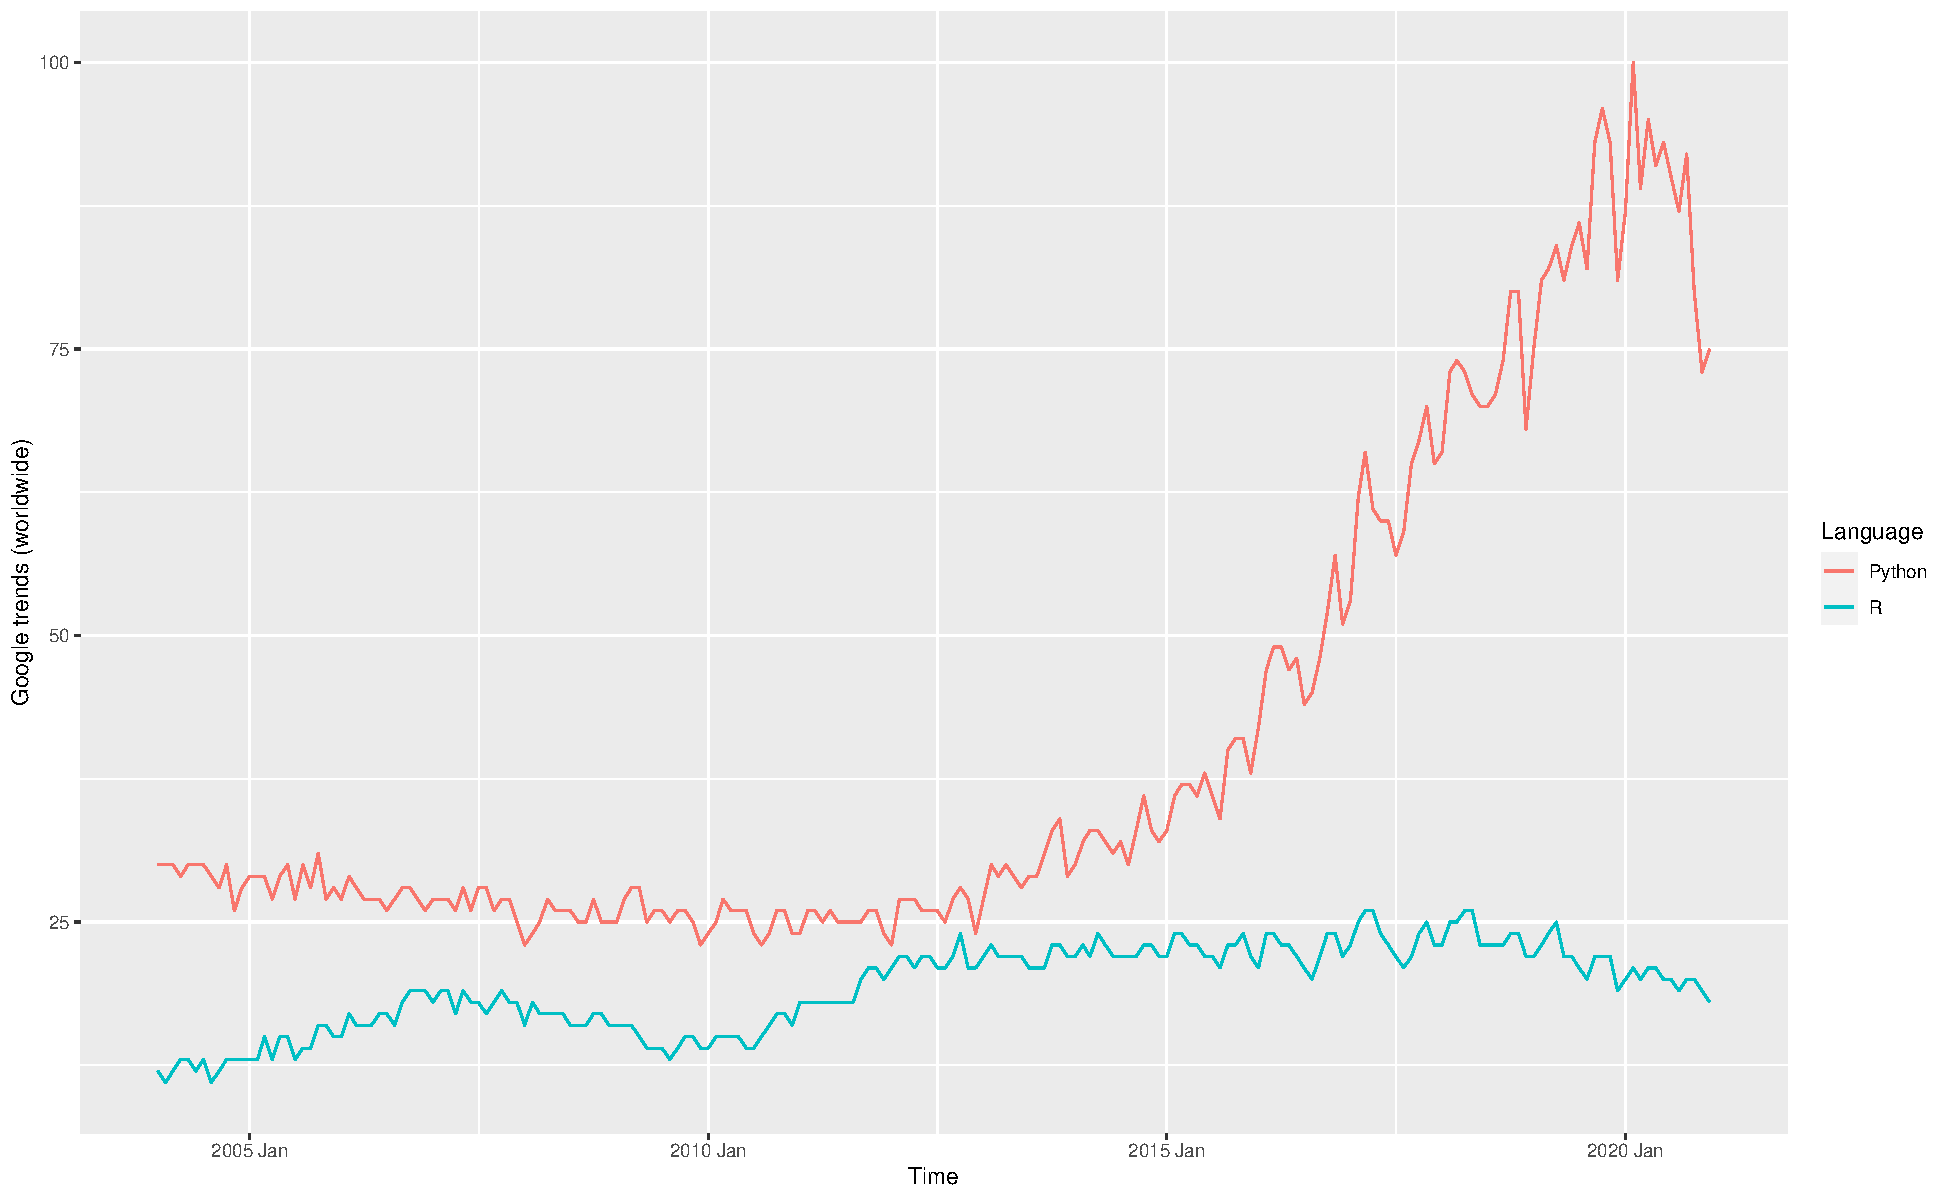
\includegraphics{IamBilingual_files/figure-latex/googletrends-1.pdf}

\hypertarget{installation}{%
\section{Installation}\label{installation}}

\hypertarget{python-3}{%
\subsection{Python}\label{python-3}}

Ref: \url{https://www.w3schools.com/python/python_getstarted.asp}

Many PCs and Macs will have python already installed.

To check if you have python installed on a Windows PC, search in the start bar for Python or run the following on the Command Line (cmd.exe):

\texttt{C:\textbackslash{}Users\textbackslash{}Your\ Name\textgreater{}python\ -\/-version}

To check if you have python installed on a Linux or Mac, then on linux open the command line or on Mac open the Terminal and type:

\texttt{python\ -\/-version}

If you find that you do not have python installed on your computer, then you can download it for free from the following website: \url{https://www.python.org/}

\hypertarget{r-3}{%
\subsection{R}\label{r-3}}

You can download it for free from the following websites:

\begin{itemize}
\tightlist
\item
  R (\url{https://cran.r-project.org/})
\item
  RStudio (\url{https://www.rstudio.com/products/rstudio/download/\#download}).
\end{itemize}

\hypertarget{ranked15python-packages}{%
\section{Ranked:15Python packages}\label{ranked15python-packages}}

for Data Science

\url{http://blog.thedataincubator.com/wp-content/uploads/2017/04/Ranked-15-Python-Packages-for-Data-Science.pdf}

\hypertarget{variables-expressions-and-statements}{%
\chapter{Variables, expressions, and statements}\label{variables-expressions-and-statements}}

\hypertarget{basic-exmaple}{%
\section{Basic Exmaple}\label{basic-exmaple}}

This is a test code

\hypertarget{r-code}{%
\subsection{R code}\label{r-code}}

\begin{Shaded}
\begin{Highlighting}[]
\CommentTok{# This is an R code}
\NormalTok{x <-}\StringTok{ }\DecValTok{1}
\NormalTok{y <-}\StringTok{ }\DecValTok{3}
\KeywordTok{print}\NormalTok{(x}\OperatorTok{+}\NormalTok{y)}
\end{Highlighting}
\end{Shaded}

\begin{verbatim}
## [1] 4
\end{verbatim}

\hypertarget{python-code}{%
\subsection{Python Code}\label{python-code}}

The `python' engine in knitr requires the \texttt{reticulate} package.

\begin{Shaded}
\begin{Highlighting}[]
\KeywordTok{library}\NormalTok{(reticulate)}
\end{Highlighting}
\end{Shaded}

\begin{Shaded}
\begin{Highlighting}[]
\CommentTok{# This is a Python code}
\NormalTok{x }\OperatorTok{=} \DecValTok{1}
\NormalTok{y }\OperatorTok{=} \DecValTok{3}
\BuiltInTok{print}\NormalTok{(x}\OperatorTok{+}\NormalTok{y)}
\end{Highlighting}
\end{Shaded}

\begin{verbatim}
## 4
\end{verbatim}

\hypertarget{conditional-execution}{%
\chapter{Conditional execution}\label{conditional-execution}}

WIP

\hypertarget{functions}{%
\chapter{Functions}\label{functions}}

WIP

\hypertarget{iteration}{%
\chapter{Iteration}\label{iteration}}

WIP

\hypertarget{import}{%
\chapter{Import}\label{import}}

WIP

\hypertarget{tidy}{%
\chapter{Tidy}\label{tidy}}

WIP

\hypertarget{transform}{%
\chapter{Transform}\label{transform}}

WIP

\hypertarget{data-visualization}{%
\chapter{Data Visualization}\label{data-visualization}}

\hypertarget{data}{%
\section{Data}\label{data}}

The Palmer penguins dataset was introduced by Allison Horst, Alison Hill, and Kristen Gorman provide a great dataset for data exploration and visualization, as an alternative to iris. It was first introduced as an R package. The released version of palmerpenguins can be instaalled from CRAN with:

\textbf{R Installation}
\texttt{install.packages("palmerpenguins")}

Using \href{https://pypi.org/project/palmerpenguins/}{\texttt{palmerpenguins} python package} you can easily load the Palmer penguins into your python environment.

\textbf{Python Installation}
\texttt{pip\ install\ palmerpenguins}

The palmerpenguins package contains two datasets : \texttt{penguins} and \texttt{penguins\_raw}. \texttt{penguins} is a simplified version of the \texttt{penguins\_raw} data.

\hypertarget{r-4}{%
\section{R}\label{r-4}}

\textbf{Load data}

\begin{Shaded}
\begin{Highlighting}[]
\CommentTok{# Load Palmer Archipelago (Antarctica) Penguin Data}
\KeywordTok{library}\NormalTok{(palmerpenguins)}
\CommentTok{# Return the first part of the dataset}
\KeywordTok{head}\NormalTok{(penguins)}
\end{Highlighting}
\end{Shaded}

\begin{verbatim}
## # A tibble: 6 x 8
##   species island bill_length_mm bill_depth_mm flipper_length_~ body_mass_g sex  
##   <fct>   <fct>           <dbl>         <dbl>            <int>       <int> <fct>
## 1 Adelie  Torge~           39.1          18.7              181        3750 male 
## 2 Adelie  Torge~           39.5          17.4              186        3800 fema~
## 3 Adelie  Torge~           40.3          18                195        3250 fema~
## 4 Adelie  Torge~           NA            NA                 NA          NA <NA> 
## 5 Adelie  Torge~           36.7          19.3              193        3450 fema~
## 6 Adelie  Torge~           39.3          20.6              190        3650 male 
## # ... with 1 more variable: year <int>
\end{verbatim}

\begin{Shaded}
\begin{Highlighting}[]
\CommentTok{# Retrieve column names}
\KeywordTok{colnames}\NormalTok{(penguins)}
\end{Highlighting}
\end{Shaded}

\begin{verbatim}
## [1] "species"           "island"            "bill_length_mm"   
## [4] "bill_depth_mm"     "flipper_length_mm" "body_mass_g"      
## [7] "sex"               "year"
\end{verbatim}

\hypertarget{base-r-package}{%
\subsection{\texorpdfstring{\texttt{base} R package}{base R package}}\label{base-r-package}}

\begin{Shaded}
\begin{Highlighting}[]
\CommentTok{# Define color for each of the 3 penguine species}
\NormalTok{colors <-}\StringTok{ }\KeywordTok{c}\NormalTok{(}\StringTok{"#00AFBB"}\NormalTok{, }\StringTok{"#E7B800"}\NormalTok{, }\StringTok{"#FC4E07"}\NormalTok{)}
\NormalTok{colors <-}\StringTok{ }\NormalTok{colors[}\KeywordTok{as.numeric}\NormalTok{(penguins}\OperatorTok{$}\NormalTok{species)]}

\CommentTok{# Define shapes}
\NormalTok{shapes =}\StringTok{ }\KeywordTok{c}\NormalTok{(}\DecValTok{16}\NormalTok{, }\DecValTok{17}\NormalTok{, }\DecValTok{18}\NormalTok{) }
\NormalTok{shapes <-}\StringTok{ }\NormalTok{shapes[}\KeywordTok{as.numeric}\NormalTok{(penguins}\OperatorTok{$}\NormalTok{species)]}

\KeywordTok{plot}\NormalTok{(}\DataTypeTok{x =}\NormalTok{ penguins}\OperatorTok{$}\NormalTok{flipper_length_mm,}
          \DataTypeTok{y =}\NormalTok{ penguins}\OperatorTok{$}\NormalTok{body_mass_g,}
          \DataTypeTok{col =}\NormalTok{ colors,}
          \DataTypeTok{pch =}\NormalTok{ shapes,}
          \DataTypeTok{xlab =} \StringTok{"Flipper Length"}\NormalTok{,}
          \DataTypeTok{ylab =} \StringTok{"Body Mass"}\NormalTok{ )}
\end{Highlighting}
\end{Shaded}

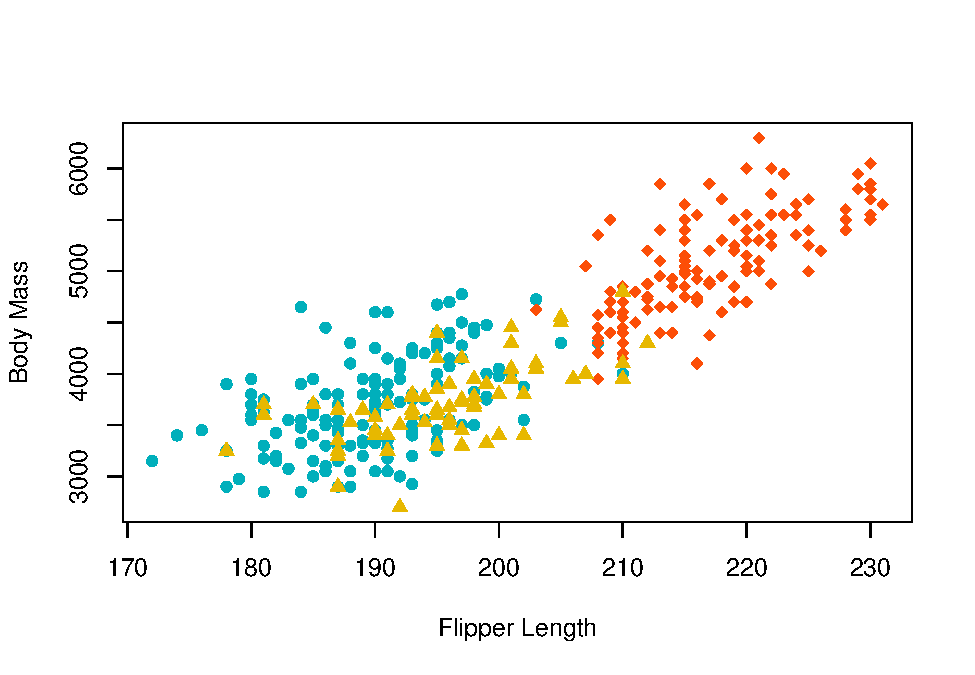
\includegraphics{IamBilingual_files/figure-latex/unnamed-chunk-6-1.pdf}

\hypertarget{gggplot2-package}{%
\subsection{\texorpdfstring{\texttt{gggplot2} Package}{gggplot2 Package}}\label{gggplot2-package}}

\texttt{ggplot2} is an R package dedicated to data visualization which is based on The Grammar of Graphics \citep{wilkinson2012grammar}.

\begin{Shaded}
\begin{Highlighting}[]
\CommentTok{#load ggplot2 package to make statistical graphics}
\KeywordTok{library}\NormalTok{(ggplot2)}
\NormalTok{p <-}\StringTok{ }\KeywordTok{ggplot}\NormalTok{(penguins) }\OperatorTok{+}
\StringTok{  }\KeywordTok{geom_point}\NormalTok{( }\KeywordTok{aes}\NormalTok{(}\DataTypeTok{x =}\NormalTok{ flipper_length_mm,}
                  \DataTypeTok{y =}\NormalTok{ body_mass_g,}
                  \DataTypeTok{color =}\NormalTok{ species,}
                  \DataTypeTok{shape =}\NormalTok{ species)) }\OperatorTok{+}
\StringTok{  }\KeywordTok{xlab}\NormalTok{(}\StringTok{"Flipper Length"}\NormalTok{)}\OperatorTok{+}
\StringTok{  }\KeywordTok{ylab}\NormalTok{(}\StringTok{"Body Mass"}\NormalTok{)}

\KeywordTok{print}\NormalTok{(p)}
\end{Highlighting}
\end{Shaded}

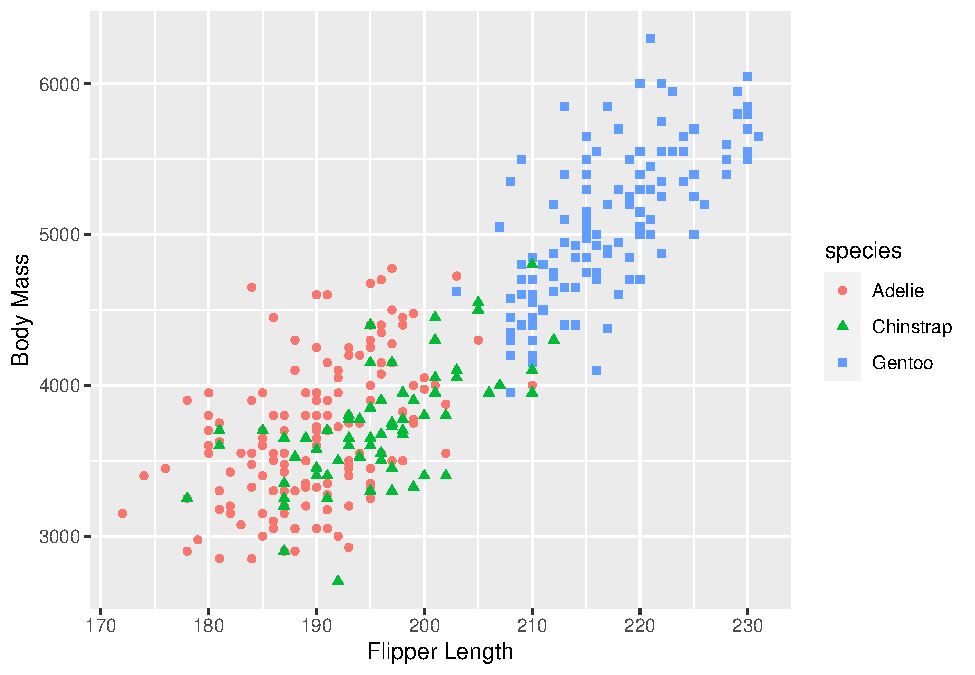
\includegraphics{IamBilingual_files/figure-latex/unnamed-chunk-7-1.pdf}

\hypertarget{plotly-r-package-for-interactive-data-visualization}{%
\subsection{\texorpdfstring{\texttt{plotly} R package for interactive data visualization}{plotly R package for interactive data visualization}}\label{plotly-r-package-for-interactive-data-visualization}}

Interactive visualization focuses on graphic representations of data that improve the way we interact with information

plotly is an R package for creating interactive web-based graphs via the open source JavaScript graphing library plotly.js.

\begin{Shaded}
\begin{Highlighting}[]
\KeywordTok{library}\NormalTok{(plotly)}
\NormalTok{p <-}\StringTok{ }\KeywordTok{ggplot}\NormalTok{(penguins) }\OperatorTok{+}
\StringTok{  }\KeywordTok{geom_point}\NormalTok{( }\KeywordTok{aes}\NormalTok{(}\DataTypeTok{x =}\NormalTok{ flipper_length_mm,}
                  \DataTypeTok{y =}\NormalTok{ body_mass_g,}
                  \DataTypeTok{color =}\NormalTok{ species,}
                  \DataTypeTok{shape =}\NormalTok{ species)) }\OperatorTok{+}
\StringTok{  }\KeywordTok{xlab}\NormalTok{(}\StringTok{"Flipper Length"}\NormalTok{)}\OperatorTok{+}
\StringTok{  }\KeywordTok{ylab}\NormalTok{(}\StringTok{"Body Mass"}\NormalTok{)}

\CommentTok{# The function ggplotly converts a ggplot2::ggplot() object to a plotly object.}
\NormalTok{plotly}\OperatorTok{::}\KeywordTok{ggplotly}\NormalTok{(p)}
\end{Highlighting}
\end{Shaded}

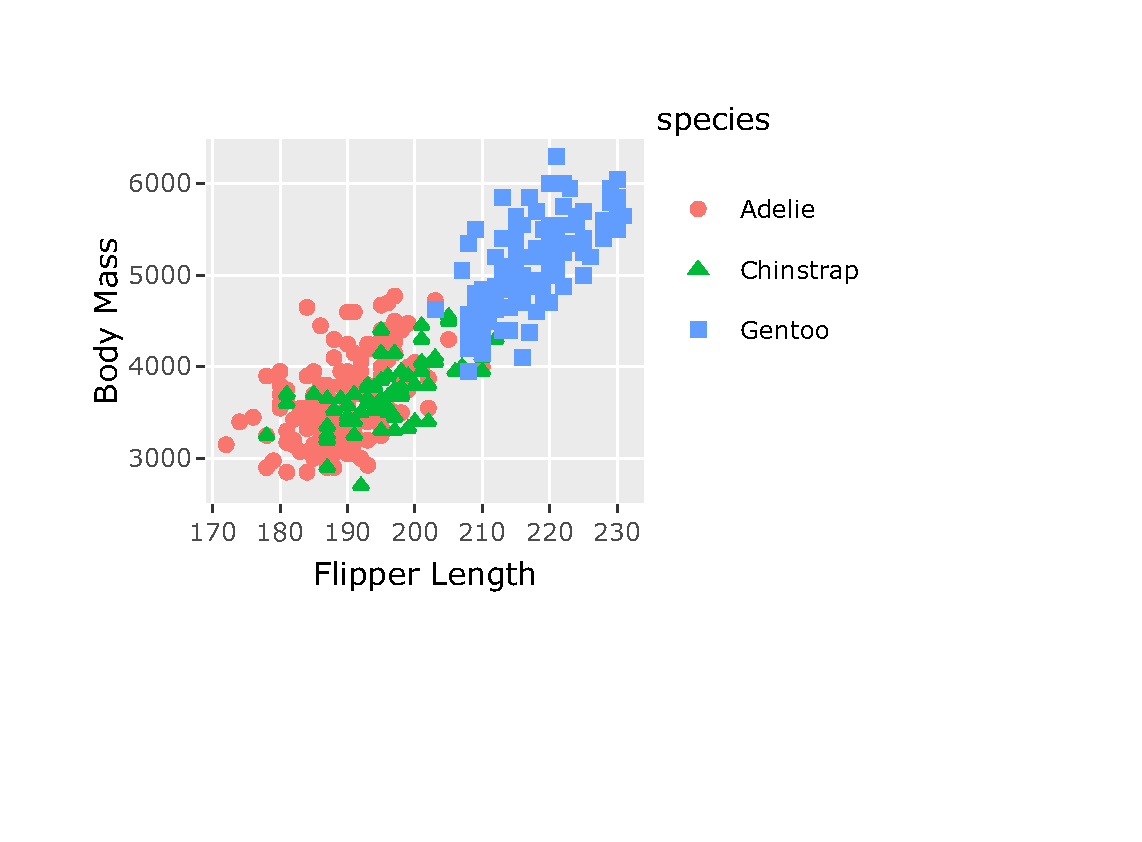
\includegraphics{IamBilingual_files/figure-latex/unnamed-chunk-8-1.pdf}

\textbf{Method 2}

\begin{Shaded}
\begin{Highlighting}[]
\KeywordTok{library}\NormalTok{(plotly)}
\NormalTok{fig <-}\StringTok{ }\KeywordTok{plot_ly}\NormalTok{(penguins, }
               \DataTypeTok{x =} \OperatorTok{~}\NormalTok{flipper_length_mm,}
               \DataTypeTok{y =} \OperatorTok{~}\NormalTok{body_mass_g, }
               \DataTypeTok{color =} \OperatorTok{~}\NormalTok{species,}
               \DataTypeTok{symbol =} \OperatorTok{~}\NormalTok{species,}
               \DataTypeTok{type =} \StringTok{"scatter"}\NormalTok{)}
\NormalTok{fig}
\end{Highlighting}
\end{Shaded}

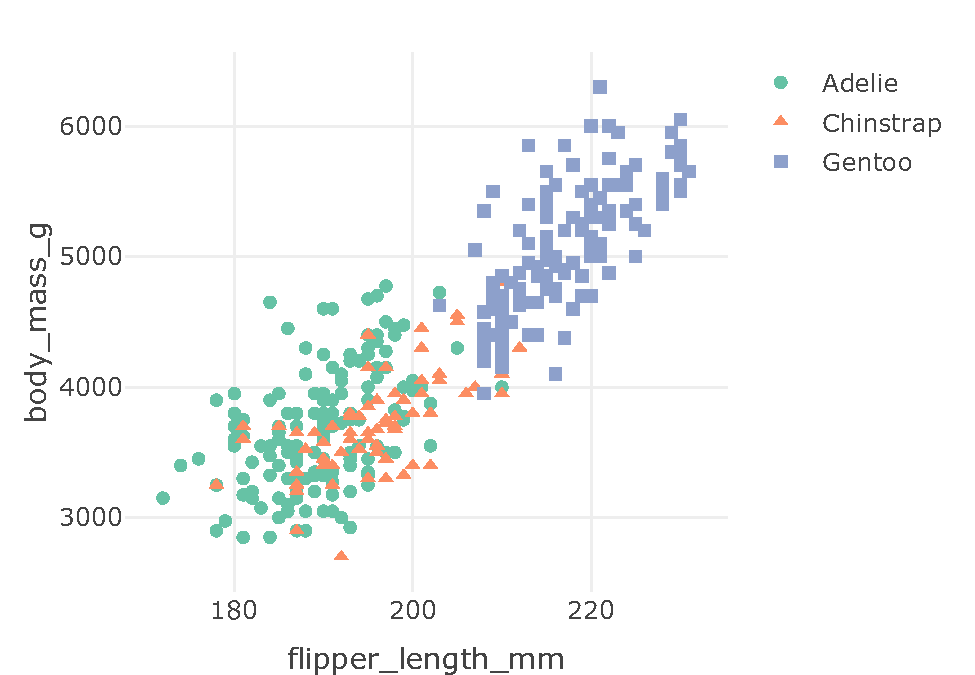
\includegraphics{IamBilingual_files/figure-latex/unnamed-chunk-9-1.pdf}

\hypertarget{python-4}{%
\section{Python}\label{python-4}}

\textbf{Load data}

\begin{Shaded}
\begin{Highlighting}[]
\CommentTok{#load functions in palmerpenguins package}
\ImportTok{from}\NormalTok{ palmerpenguins }\ImportTok{import}\NormalTok{ load_penguins}
\NormalTok{penguins }\OperatorTok{=}\NormalTok{ load_penguins()}
\CommentTok{# Return the first part of the dataset}
\NormalTok{penguins.head()}
\CommentTok{# Retrieve column names}
\BuiltInTok{list}\NormalTok{(penguins.columns)}
\end{Highlighting}
\end{Shaded}

\hypertarget{matplotlib-package}{%
\subsection{\texorpdfstring{\texttt{Matplotlib} package}{Matplotlib package}}\label{matplotlib-package}}

Matplotlib is mainly deployed for basic plotting. Visualization using Matplotlib generally consists of bars, pies, lines, scatter plots and so on.

\begin{Shaded}
\begin{Highlighting}[]
\CommentTok{# Import matplotlib to make statistical graphics. }
\CommentTok{# By convention, it is imported with the shorthand sns.}
\ImportTok{import}\NormalTok{ matplotlib.pyplot }\ImportTok{as}\NormalTok{ plt}

\NormalTok{colors }\OperatorTok{=}\NormalTok{ \{}\StringTok{'Adelie'}\NormalTok{:}\StringTok{'blue'}\NormalTok{, }\StringTok{'Gentoo'}\NormalTok{:}\StringTok{'orange'}\NormalTok{, }\StringTok{'Chinstrap'}\NormalTok{:}\StringTok{'green'}\NormalTok{\}}
\NormalTok{plt.scatter(penguins.flipper_length_mm,}
\NormalTok{penguins.body_mass_g, }
\NormalTok{c}\OperatorTok{=}\NormalTok{ penguins.species.}\BuiltInTok{apply}\NormalTok{(}\KeywordTok{lambda}\NormalTok{ x: colors[x]))}
\NormalTok{plt.xlabel(}\StringTok{'Flipper Length'}\NormalTok{)}
\NormalTok{plt.ylabel(}\StringTok{'Body Mass'}\NormalTok{)}
\end{Highlighting}
\end{Shaded}

\begin{center}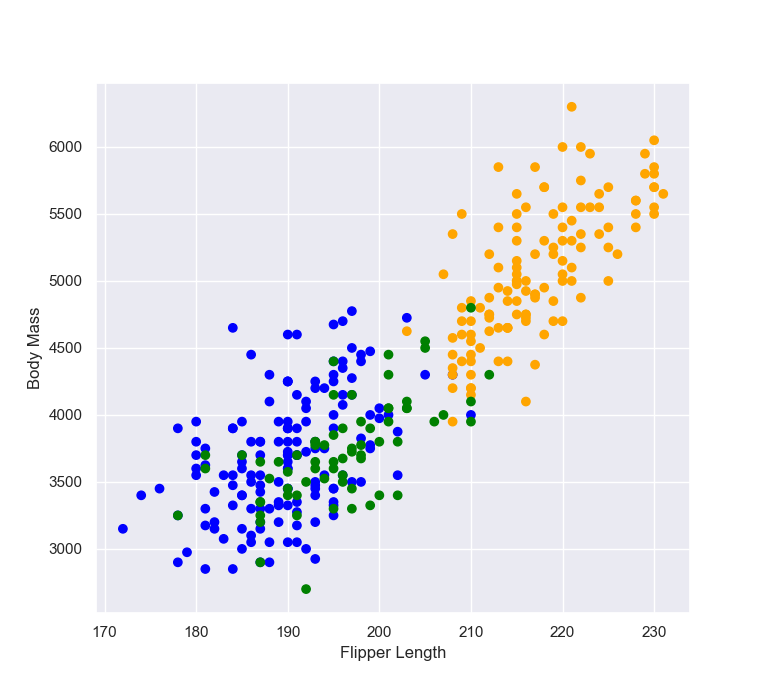
\includegraphics[width=0.9\linewidth]{fig/Viz_chap/1_matplot} \end{center}

\hypertarget{seaborn-package}{%
\subsection{\texorpdfstring{\texttt{seaborn} Package}{seaborn Package}}\label{seaborn-package}}

Seaborn provides a variety of visualization patterns. It uses fewer syntax and has easily interesting default themes.

\begin{Shaded}
\begin{Highlighting}[]
\CommentTok{# Import seaborn to make statistical graphics. }
\CommentTok{# By convention, it is imported with the shorthand sns.}
\ImportTok{import}\NormalTok{ seaborn }\ImportTok{as}\NormalTok{ sns }
\CommentTok{#load functions in palmerpenguins package}
\ImportTok{from}\NormalTok{ palmerpenguins }\ImportTok{import}\NormalTok{ load_penguins}
\NormalTok{penguins }\OperatorTok{=}\NormalTok{ load_penguins()}

\CommentTok{# Apply the default theme}
\NormalTok{sns.set_theme()}
\CommentTok{# sns.set_style('whitegrid')}
\NormalTok{p }\OperatorTok{=}\NormalTok{ sns.relplot(x }\OperatorTok{=} \StringTok{'flipper_length_mm'}\NormalTok{,}
\NormalTok{            y }\OperatorTok{=}\StringTok{'body_mass_g'}\NormalTok{,}
\NormalTok{            hue }\OperatorTok{=} \StringTok{'species'}\NormalTok{,}
\NormalTok{            style }\OperatorTok{=} \StringTok{'species'}\NormalTok{,}
\NormalTok{            data }\OperatorTok{=}\NormalTok{ penguins)}
\NormalTok{p.set_xlabels(}\StringTok{'Flipper Length'}\NormalTok{)}
\NormalTok{p.set_ylabels(}\StringTok{'Body Mass'}\NormalTok{)   }
\end{Highlighting}
\end{Shaded}

\begin{center}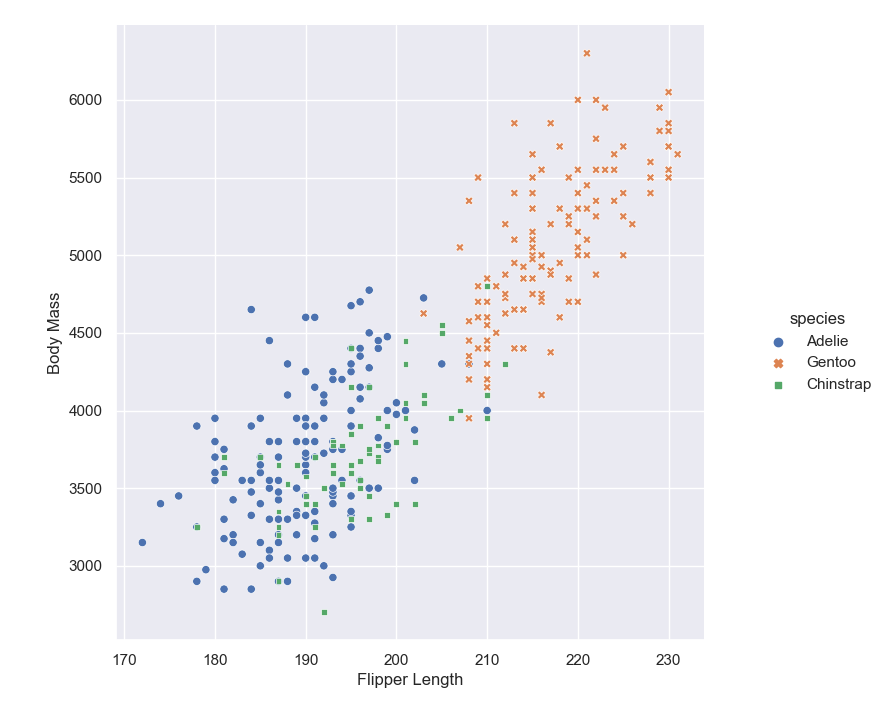
\includegraphics[width=0.9\linewidth]{fig/Viz_chap/2_seaborn} \end{center}

The function \texttt{relplot()} is named that way because it is designed to visualize many different statistical relationships. The \texttt{relplot()} function has a convenient kind parameter that lets you easily switch to this alternate representation:
\texttt{scatterplot()} with \texttt{kind="scatter"}; the default and \texttt{lineplot()} with \texttt{kind="line"}.

\hypertarget{plotnine-package}{%
\subsection{\texorpdfstring{\texttt{plotnine} package}{plotnine package}}\label{plotnine-package}}

\url{https://pypi.org/project/plotnine/}

plotnine is an implementation of a grammar of graphics in Python, it is based on ggplot2. The grammar allows users to compose plots by explicitly mapping data to the visual objects that make up the plot.

Plotting with a grammar is powerful, it makes custom (and otherwise complex) plots are easy to think about and then create, while the simple plots remain simple.

\textbf{NOTE: R vs Python Syntax}

\textbf{Unlike in R, now all the variables must be enclosed by single quotes}

\begin{Shaded}
\begin{Highlighting}[]
\ImportTok{from}\NormalTok{ plotnine }\ImportTok{import} \OperatorTok{*}
\CommentTok{# unlike in R, now all the variables must be enclosed by single quotes}
\NormalTok{(ggplot(penguins) }\OperatorTok{+}
\NormalTok{  geom_point(aes(x }\OperatorTok{=} \StringTok{'flipper_length_mm'}\NormalTok{,}
\NormalTok{                  y }\OperatorTok{=} \StringTok{'body_mass_g'}\NormalTok{,}
\NormalTok{                  color }\OperatorTok{=} \StringTok{'species'}\NormalTok{,}
\NormalTok{                  shape }\OperatorTok{=} \StringTok{'species'}\NormalTok{)) }\OperatorTok{+}
\NormalTok{  xlab(}\StringTok{"Flipper Length"}\NormalTok{)}\OperatorTok{+}
\NormalTok{  ylab(}\StringTok{"Body Mass"}\NormalTok{))}
\end{Highlighting}
\end{Shaded}

\begin{center}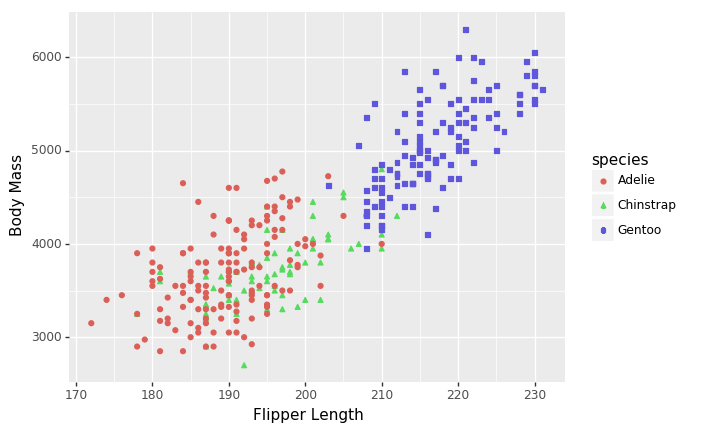
\includegraphics[width=0.9\linewidth]{fig/Viz_chap/3_plotnine} \end{center}

\hypertarget{plotly-python-library-for-interactive-data-visualization}{%
\subsection{\texorpdfstring{\texttt{plotly} Python library for interactive data visualization}{plotly Python library for interactive data visualization}}\label{plotly-python-library-for-interactive-data-visualization}}

The \texttt{plotly.express} (Plotly Express or PX) module contains functions that can create entire figures at once. It is usually imported as \texttt{px}. Plotly Express is a built-in part of the \texttt{plotly} library.

\begin{Shaded}
\begin{Highlighting}[]
\ImportTok{import}\NormalTok{ plotly.express }\ImportTok{as}\NormalTok{ px}

\NormalTok{fig }\OperatorTok{=}\NormalTok{ px.scatter(penguins,}
\NormalTok{                 x}\OperatorTok{=}\StringTok{"flipper_length_mm"}\NormalTok{,}
\NormalTok{                 y}\OperatorTok{=}\StringTok{"body_mass_g"}\NormalTok{,}
\NormalTok{                 color}\OperatorTok{=} \StringTok{"species"}\NormalTok{,}
\NormalTok{                 symbol}\OperatorTok{=} \StringTok{"species"}\NormalTok{,}
\NormalTok{                 labels}\OperatorTok{=}\BuiltInTok{dict}\NormalTok{(flipper_length_mm}\OperatorTok{=}\StringTok{"Flipper Length"}\NormalTok{,}
\NormalTok{                             body_mass_g}\OperatorTok{=}\StringTok{"Body Mass"}\NormalTok{))}
\NormalTok{fig.show()}
\end{Highlighting}
\end{Shaded}

\hypertarget{model}{%
\chapter{Model}\label{model}}

WIP

\hypertarget{communicate}{%
\chapter{Communicate}\label{communicate}}

WIP

\hypertarget{advanced-r-and-python}{%
\chapter{Advanced R and Python}\label{advanced-r-and-python}}

WIP

\hypertarget{time-series-forecasting}{%
\section{Time Series Forecasting}\label{time-series-forecasting}}

\begin{longtable}[]{@{}ll@{}}
\toprule
\begin{minipage}[b]{0.47\columnwidth}\raggedright
R\strut
\end{minipage} & \begin{minipage}[b]{0.47\columnwidth}\raggedright
Python\strut
\end{minipage}\tabularnewline
\midrule
\endhead
\begin{minipage}[t]{0.47\columnwidth}\raggedright
\href{https://cran.r-project.org/web/packages/fable/index.html}{fable}-Forecasting Models for Tidy Time Series\strut
\end{minipage} & \begin{minipage}[t]{0.47\columnwidth}\raggedright
\href{https://www.statsmodels.org/devel/user-guide.html\#time-series-analysis}{statsmodels}- Statistics based models\strut
\end{minipage}\tabularnewline
\begin{minipage}[t]{0.47\columnwidth}\raggedright
\href{https://cran.r-project.org/web/packages/forecast/index.html}{forecast}- Forecasting Functions for Time Series and Linear Models\strut
\end{minipage} & \begin{minipage}[t]{0.47\columnwidth}\raggedright
\href{https://www.sktime.org/en/latest/}{sktime}- A unified framework for machine learning with time series\strut
\end{minipage}\tabularnewline
\begin{minipage}[t]{0.47\columnwidth}\raggedright
\(\text{}\)\strut
\end{minipage} & \begin{minipage}[t]{0.47\columnwidth}\raggedright
\href{https://ts.gluon.ai/}{GluonTS}- Deep learning-based models.\strut
\end{minipage}\tabularnewline
\bottomrule
\end{longtable}

\bibliography{book.bib}

\end{document}
